\documentclass[]{article}

% Imported Packages
%------------------------------------------------------------------------------
\usepackage{amssymb}
\usepackage{amstext}
\usepackage{amsthm}
\usepackage{amsmath}
\usepackage{enumerate}
\usepackage{fancyhdr}
\usepackage[margin=1in]{geometry}
\usepackage{graphicx}
\usepackage{extarrows}
\usepackage{setspace}
\usepackage[section]{placeins}
\usepackage{float}
\usepackage[utf8]{inputenc}
\usepackage{hyperref}


%------------------------------------------------------------------------------

% Header and Footer
%------------------------------------------------------------------------------
\pagestyle{plain}  
\renewcommand\headrulewidth{0.4pt}                                      
\renewcommand\footrulewidth{0.4pt}                                    
%------------------------------------------------------------------------------

% Title Details
%------------------------------------------------------------------------------
\title{iSpaceship - Deliverable 1}
\author{SE 3A04: Software Design II -- Large System Design}
\author{Team
		\\ Pedram Yazdinia, yazdinip
		\\ Will Conry, conrywm
		\\ Torja Istiaque, istiaqum
		\\ Akila Kavisinghe, kavisina
		\\ Xiangxin Kong, kongx9
}

\date{\today}
                            
%------------------------------------------------------------------------------

% Document
%------------------------------------------------------------------------------
\begin{document}

\newpage

\maketitle	
\tableofcontents
\newpage
\section{Introduction}
\label{sec:introduction}
% Begin Section

%\textbf{This section of the SRS should provide an overview of the entire SRS. }

This document is intended to provide a general overview of the requirements specifications for the video game \textit{iSpaceship}. The document is organized with the following sections in this order: Introduction, Scope, Overall Description, Use Case Diagram, Functional Requirements, and Non-functional Requirements. 

\subsection{Purpose}
\label{sub:purpose}
% Begin SubSection
    %a) Delineate the purpose of the SRS
    %b) Specify the intended audience for the SRS
	The purpose of the software requirement specification is to provide a detailed overview of the software product being designed. The SRS will contain all measurable parameters and goals of the project. The document will also describe functional and non-functional requirements as well as the various stakeholders and users.
	
	This document is intended for developers, testers, and project managers within the group including the TA’s and the professor. Developers will refer to the document at each stage of the design process in order to meet the design requriments. 
	

% End SubSection

\subsection{Scope}
\label{sub:scope}
% Begin SubSection
%\begin{enumerate}[a)]
	%\item \textbf{Identify the software product(s) to be produced by name (e.g., Host DBMS, Report Generator, etc.)}
	%\item \textbf{Explain what the software product(s) will, and, if necessary, will not do}
	%\item \textbf{Describe the application of the software being specified, including relevant benefits, objectives, and goals}
	%\item \textbf{Be consistent with similar statements in higher-level specifications (e.g., the system requirements specification), if they exist}
	
	
 “iSpaceship” is a Rogue-like, turn-based, spaceship battle simulator, desktop video game. The software product will provide the user with an engaging gaming experience where they can build their own spaceship, face disasters, and battle other spaceships. 	The software product will be used for the enjoyment of the user and provide them with a sense of self-accomplishment. The objective is for users to have fun and feel rewarded when they put in the time and dedication to progress in the game. The application should hold interest of users over a long period of time.
	

%\end{enumerate}
% End SubSection

\subsection{Definitions, Acronyms, and Abbreviations}
\label{sub:definitions_acronyms_and_abbreviations}
% Begin SubSection
\begin{enumerate}[a)]
	%\item \textbf{Provide the definitions of all terms, acronyms, and abbreviations required to properly interpret the SRS}
	
	\item Rogue-Like - Video game genre where players restart completely upon permanent death of the player character.
 
    \item Turn-Based - Strategy game where players take turns playing.
    
    \item Gamer - A person who is enthusiastic about video games. 
    
    \item AWS - Amazon Web Services
    
    \item XP - Points associated to the progress of the player in the game 
    
    \item Ability - Abilities are special powers that allows each spaceship to battle with other spaceships.
    
	\item Components - Each component is used to improve the power that comes along with each ability. 
	
\end{enumerate}
% End SubSection

\subsection{References}
\begin{enumerate}
    \item SE3A04 tutorial slides2 and slides3 by Andrew LeClair
    \item Unity documentation, available at: \url{https://docs.unity3d.com/}
\end{enumerate}
\label{sub:references}
% Begin SubSection
%\begin{enumerate}[a)]
%	\item \textbf{Provide a complete list of all documents referenced elsewhere in the SRS}
%	\item \textbf{Identify each document by title, report number (if applicable), date, and publishing organization}
%	\item \textbf{Specify the sources from which the references can be obtained}
%\end{enumerate}
% End SubSection

\subsection{Overview}
\label{sub:overview}
% Begin SubSection
%\begin{enumerate}[a)]
%	\item \textbf{Describe what the rest of the SRS contains}
%	\item Explain how the SRS is organized
	This document encapsulates critical information which will be used as a foundation of the entire project. This document first discusses the general factors that affect the product and the requirements. This information enables the reader to have a better grasp and understanding on the requirements that come after. These factors include product perspective product functions, user characteristics and constraints. The reader is then presented with a Use Case diagrams which visually shows the interaction between different actors and tasks. The largest portion of the document is then dedicated to clearly stating and explaining the functional and non-functional requirements. Attached at the end is a spreadsheet that shows the division of labour within the team. 
%\end{enumerate}
% End SubSection

% End Section

\section{Overall Description}
\label{sec:overall_description}
% Begin Section

This section of the SRS will describe the general factors that affect the product and its requirements. It does not state specific requirements; it provides a background for those requirements and makes them easier to understand. It will also describes functionalities guaranteed for each stakeholder, in addition to constraints and assumptions that affect the overview of the system. 

\subsection{Product Perspective}

% Begin SubSection

    Inspired by retro spaceship game Galaxia, which was published in 1970's by Bandai Namco, iSpaceship will be made up of an single player component as well as a multiplayer component. While the single player component is self contained as it only consists of the interactions between the player and the "AI" driven bots, the multiplayer component takes advantage of a server that is used to sync the game at all times. Doing so allows for both online and offline multiplayer as one of the desktops can also act as the server and the players would then play using LAN. An online server can also be used which gives the option to play with any one who has an internet connection, allowing players to play over any distance. 
    
    
\label{sub:product_perspective}
%\begin{enumerate}[a)]    
	%\item \textbf{Put the product into perspective with other related products, i.e., context}
	%\item If the product is independent and totally self-contained, it should be stated here
	%\item If the SRS defines a product that is a component of a larger system, as frequently occurs, then this subsection should relate the requirements of that larger system to functionality of the software and should identify interfaces between that system and the software
	%\item A block diagram showing the major components of the larger system, interconnections, and external interfaces can be helpful
%\end{enumerate}
% End SubSection

\subsection{Product Functions}
\label{sub:product_functions}
% Begin SubSection
% everyone has 3 lives 
% if you lose all you lose everything
% if you finish story mode, you have option of going back to level 0 
%write down functionality of battle
%have drops 


The system's functionality is centralized around the user upgrading their spaceship so that they are able to eventually complete the story mode. An experience level will be assigned to a user's spaceship based on their statistics, initially level 1. These statistics will improve as the user progresses thorough the story. Upgrades will be purchased with in-game currency and will come in the form of components. Purchasing of components will be made available through the shop. Components will augment the spaceships' abilities which are used in battle. In-game currency can be attained through winning battles or over time through the money generator. Battles involve the user's spaceship trying to eliminate an opponent's spaceship by using their abilities in a turn based fashion. Opponents will take the form of bots  in the case of story mode, and other users in the case of multiplayer mode. Winning battles will result in in-game currency and XP being awarded to the user, losing 3 story mode battles will result in the user starting back to their base ship at level 1. Finally the user will be able to navigate through the shop, the story mode, and multiplayer mode.  
%regression through either battle or a random event?, does regression have to always occur 
%once you beat the game you start from the beg ginning
%should i aggregate the currency and abilities?
% should i describe the battle mechanic; how stats and abilities come to play 

%\begin{enumerate}[a)]
%	\item Provide a summary of the major fufnctions that the software will perform.
%	\begin{itemize}
		%\item \textbf{Example}: An SRS for an accounting program may use this part to address customer account maintenance, customer statement, and invoice preparation without mentioning the vast amount of detail that each of those functions requires.
%	\end{itemize}
%	\item Functions should be organized in a way that makes the list of functions understandable to the customer or to anyone else reading the document for the first time
%	\item Textual or graphical methods can be used to show the different functions and their relationships
	%\begin{itemize}
%		\item Such a diagram is not intended to show a design of a product, but simply shows the logical relationships among variables
%	\end{itemize} 
%\end{enumerate}
% End SubSection

\subsection{User Characteristics}
\label{sub:user_characteristics}
% Begin SubSection

	%\item Describe those general characteristics of the intended users of the product including educational level, experience, and technical expertise
	
	The game is intended for users of all ages and education levels. The game is run on a computer running Windows or Mac OS X, so basic technical knowledge of either operating system is required to install the game. Understanding written English is beneficial as well because the instructions and menu items are in English. The game is intended for players with any level of video game experience.
	
	%\item Do not state specific requirements, but rather provide the reasons why certain specific requirements are later specified
	To facilitate this: The game must be appropriate for all ages. The installer will be simple enough for someone inexperienced with computers to use. The interface must be intuitive so that it can be quickly learned. To keep it interesting for players with varying levels of experience the game will progressively become more challenging.

% End SubSection

\subsection{Constraints}
\label{sub:constraints}
% Begin SubSection
\begin{enumerate}

	% Provide a general description of any other items that will limit the developer's options
    \item \textbf{Operating System}: The game is only intended for use on either Windows or Mac OS X.
	\item \textbf{Game Engine}: The developers are constrained to using the Unity game engine. 
	\item \textbf{Input}: The only input methods allowed are with a cursor (mouse/trackpad) and a keyboard, touchscreen will not be supported. 
	\item \textbf{Networking}: Multiplayer functionality will use AWS for a web server to host the game.

	
	
\end{enumerate}

% End SubSection

\subsection{Assumptions and Dependencies}
\label{sub:assumptions_and_dependencies}
% Begin SubSection
\begin{enumerate}
	%\item List each of the factors that affect the requirements stated in the SRS
	%\item These factors are not design constraints on the software but are, rather, any changes to them that can affect the requirements in the SRS
		%\item \textbf{Example}: An assumption may be that a specific operating system will be available on the hardware designated for the software product. If, in fact, the operating system is not available, the SRS would then have to change accordingly.
	\item \textbf{Hardware}: It is assumed that the target demographic has access to traditional computers with a mouse and keyboard.
	\item \textbf{Game Engine}: It is assumed that the Unity game engine will be available for the developers. 
	\item \textbf{Operating System}: It is assumed that Windows and Mac OS X will be available for both the developers and users of the game.
	\item \textbf{Web Server}: It is assumed that the AWS will be available to host the servers required for multiplayer.
	
\end{enumerate}
% End SubSection

\subsection{Apportioning of Requirements}
\label{sub:apportioning_of_requirements}
% Begin SubSection
\begin{enumerate}[a)]
	\item The game will only be made in English. %versions of the system
\end{enumerate}
% End SubSection

% End Section
%
\section{Use Case Diagram}
\label{sec:use_case_diagram}
% Begin Section
%This section should provide a use case diagram for your application. 
%Each use case appearing in the diagram should be accompanied by a text description. 



\begin{center}
\begin{tabular}{ |p{5cm}|p{9cm}| } 
\hline
\textbf{Use Case} & \textbf{Description} \\ 
 \hline
Start Application & How the user initiates the system.\\
 \hline
Enter Main Menu & How the user can load the game.\\
\hline
Load Profile & User loads existing game state.\\
\hline
Change Settings & User can change in-game settings\\
\hline
Create Profile & User can create a new game state.\\
\hline
Delete Profile & User can delete an existing game state.\\
\hline
Enter Hub & Main game screen where user can do various tasks.\\
\hline
Choose Mission & Where user selects their battles.\\
\hline
Play Previous & User can play a previously played mission.\\
\hline
Continue Story & User can continue the story where they left off.\\
\hline
Battle & User engages in a battle against AI spaceship.\\
\hline
Check Stats & User can check stats of enemy spaceship and their own.\\
\hline
Play Turn & User can make a move on their opponent on their turn.\\
\hline
Basic Attack & Users does flat damage attack.\\
\hline
Ability (Battle) & User uses an ability\\
\hline
Ability Cooldown & Ability cannot be used for several turns.\\
\hline
Skip turn & User can choose to let their opponent go.\\
\hline
Shop & Where user receives items for upgrades.\\
\hline
Buy & User can buy items.\\
\hline
Ability(Buy) & User buys new ability.\\
\hline
Generator Upgrade & User can upgrades their currency generators.\\
\hline
Ability Upgrade & User can upgrade power of existing ability.\\
\hline
Quit Game & User chooses to close application.\\
\hline
Auto Save & System prompts an autosave.\\
\hline
Select Overwrite & User selects an existing profile to overwrite save.\\
\hline
\end{tabular}
\end{center}

\begin{figure}[H]
    \centering
    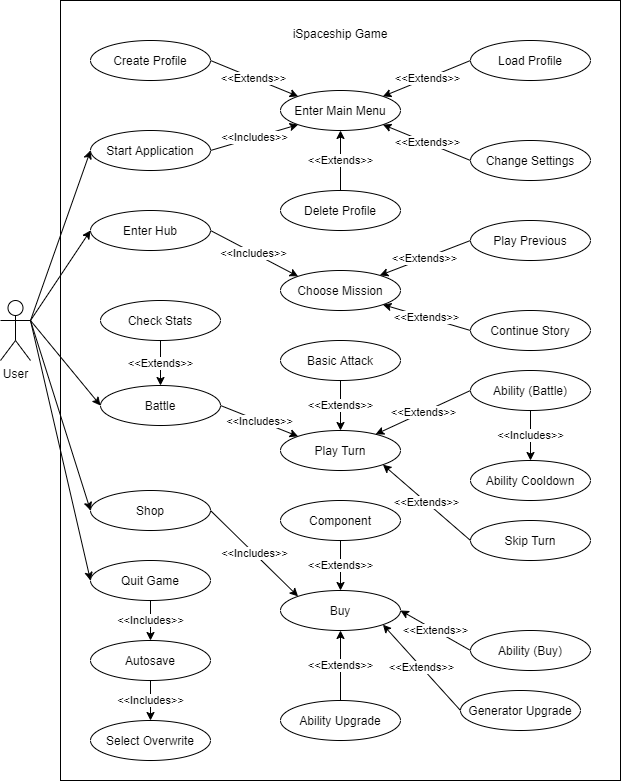
\includegraphics[width=\textwidth]{UseCaseDiagram2.png}
    \caption{Use case diagram for the iSpaceship game.}
    %\label{fig:mesh1}
\end{figure}

% End Section

\section{Functional Requirements}
\label{sec:functional_requirements}
% Begin Section



%View points: end users as anyone playing the game 

%health bar; health points in a battle 
%armour bar; defense points in a battle that user has to damage first 

%component effects stats of the moves 

%heal moves; increases hp 
%damage moves; damages opponent
%dodge moves; increases opponents chance of miss
%stun moves; percentage chance of skipping opps next move

%Stats of the spaceship increase by level.
%in each mission, the spaceship is given a health bar and armor bar. These two upgrade as level increases. The "shop" allows u to buy an upgrade for the moves available or completely new moves. There won't change stats associated to the spaceship, the stats are assoiated to each ability. For the spaceship, we only have the level which goes up by going through the game. As level increases, the initial armor and health bar in the game increase. % - User buys an item to upgrade their money generation



\begin{enumerate}[{VP}1.]
	\item User 
	\begin{enumerate}[{BE1}.1]
	
	    \item The user starts the application.
	    \begin{enumerate}
	        \item The system shall allow the user to start a new game. 
	        \item The system shall allow the user to change the settings of the game.
	        \item The system shall allow the user to load an existing profile.
	        \item The system shall allow the user to play multiplayer through a connection.
	    \end{enumerate}
	    
		 
		\item The user wants to create a new profile.
		\begin{enumerate}
			\item The user is allowed to change the default name of the spaceship.
			\item The user is allowed to choose the colour of the spaceship.
			\item The system shall prompt the user for confirmation of profile details (color and username).
			\item The system must allow the user to cancel the process.
			\item The system must present the new user with the backstory and then starts the first mission.
		\end{enumerate}
	
		
		\item The user wants to buy a component/ability.
		\begin{enumerate}
		    \item The system shall allow the user to buy components to upgrade abilities. 
		    \item The system shall update the stats of said ability, considering the component bought. 
		    \item The system shall allow the user to buy new abilities. 
		    \item The system shall update the deck of abilities available to the user. 
		    \item The system shall unlock the components specific to the newly bought abilities. 
		    \item The system shall allow the user to buy power ups that can increase the money generation or XP gain for a period of time. 

		\end{enumerate}	
		
		\item The user starts a mission. 
		\begin{enumerate}
		    \item The system shall present the user with the battle map depending on the mission. 
		    \item The system must allow the user to choose a difficulty.
            \item Upon victory, the system shall congratulate the user and unlock the next level. 
            \item The system shall reward the user with XP and in-game currency. 
            \item Upon defeat, the system must take away one health slot from the user.%, capped by a number. 
            \item The system must display the abilities of the spaceship to the user.
            %\item The system must allow the user to skip their turn.
            \item The system shall display the user's and opponent's spaceship.
            \item The system must allow the user to choose a number of abilities available from the deck, only at the start of the mission. 
            \item On the user's turn, the system must allow the user to choose an ability from the selected deck.
            \item The system must control the opponent's spaceship, given it's the opponent's turn. 
            \item Upon a mission completion, the system shall improve the opponent's spaceship
		\end{enumerate}
		

		\item The user selects an ability in a mission.
		\begin{enumerate}
		    \item The system shall render an animation that represents the ability used. 
		    \item The health of the player and opponent is modified accordingly in response to the ability.
		    \item The system must deny any access to a used ability for a period of time. 
		    \item The system must calculate and show the effect of an ability used.
		\end{enumerate}
		
		\item A discrete-time step has passed in the game.
		\begin{enumerate}
		    \item The user receives a small amount of currency.
		    \item The system shall display an updated version of the spaceship upon hitting a certain level. 
		    \item Upon each level increase, the system must increase the health and armor bar given to the user. 
		    \item The system must eliminate the spaceship if the user loses more than 3 battles. 
		    \item Upon elimination, the system must restart the user's spaceship; returning the spaceship to level 0 and only having access to the first mission.
		    \item The system shall automatically save the game. 
		   
		\end{enumerate}
		\item The user wants to start a multiplayer game.  
		    \begin{enumerate}
		        \item The system shall allow the user to create an online username.
		        \item The system shall allow the user to establish a connection to a specific server. 
		        \item The system shall randomly select a player for the first turn.  
		    \end{enumerate}
	\end{enumerate}
\end{enumerate}
% End Section

\section{Non-Functional Requirements}
\label{sec:non-functional_requirements}
% Begin Section
\subsection{Look and Feel Requirements}
\label{sub:look_and_feel_requirements}
% Begin SubSection

\subsubsection{Appearance Requirements}
\label{ssub:appearance_requirements}
% Begin SubSubSection
\begin{enumerate}[{LF}1. ]
	\item The system shall use a minimalist design.
	\item The spaceship shall be two-dimensional in design.
	\item The game will be futuristic and rustic in design.
\end{enumerate}
% End SubSubSection

\subsubsection{Style Requirements}
\label{ssub:style_requirements}
% Begin SubSubSection
\begin{enumerate}[{LF}1. ]
	\item The game will be two dimensional.
	\item The game will follow standard C/C++ coding structure.
\end{enumerate}
% End SubSubSection

% End SubSection

\subsection{Usability and Humanity Requirements}
\label{sub:usability_and_humanity_requirements}
% Begin SubSection

\subsubsection{Ease of Use Requirements}
\label{ssub:ease_of_use_requirements}
% Begin SubSubSection
\begin{enumerate}[{UH}1. ]
	\item The user shall only be prompted when decisions or confirmation are necessary.
	\item The game state must be saved automatically upon the end of each battle.
\end{enumerate}
% End SubSubSection

\subsubsection{Personalization and Internationalization Requirements}
\label{ssub:personalization_and_internationalization_requirements}
% Begin SubSubSection
\begin{enumerate}[{UH}1. ]
	\item The game shall be available in several languages.
	\item The hub can be fully customized.
\end{enumerate}
% End SubSubSection

\subsubsection{Learning Requirements}
\label{ssub:learning_requirements}
% Begin SubSubSection
\begin{enumerate}[{UH}1. ]
	\item Users can formulate their own unique play styles.
	\item Users can formulate their own battle strategies.
	\item Users will lay the foundation of a game meta.
\end{enumerate}
% End SubSubSection

\subsubsection{Understandability and Politeness Requirements}
\label{ssub:understandability_and_politeness_requirements}
% Begin SubSubSection
\begin{enumerate}[{UH}1. ]
    \item The game instructions and given button shall be easy to understand and approachable.
	\item The user with no gaming experience can learn battle mechanism after one round.
	
\end{enumerate}
% End SubSubSection

\subsubsection{Accessibility Requirements}
\label{ssub:accessibility_requirements}
% Begin SubSubSection
\begin{enumerate}[{UH}1. ]
	\item The game shall be accessible for deaf users.
	\item This game shall be playable by individuals with at least one functioning hand.
	\item The game will be playable by individuals with colour blindness.
\end{enumerate}
% End SubSubSection

% End SubSection

\subsection{Performance Requirements}
\label{sub:performance_requirements}
% Begin SubSection

\subsubsection{Speed and Latency Requirements}
\label{ssub:speed_and_latency_requirements}
% Begin SubSubSection
\begin{enumerate}[{PR}1. ]
	\item The system will allow at least 20 users play online simultaneously.
	\item Any valid user input shall receive an immediate response by the game in a manner instantaneous to the user’s perception (under 50ms).
	\item Game initialization upon opening the application shall be less than 10 seconds.
\end{enumerate}
% End SubSubSection

\subsubsection{Precision or Accuracy Requirements}
\label{ssub:precision_or_accuracy_requirements}
% Begin SubSubSection
\begin{enumerate}[{PR}1. ]
	\item All stats of spaceships must be an integer value.
\end{enumerate}
% End SubSubSection

\subsubsection{Reliability and Availability Requirements}
\label{ssub:reliability_and_availability_requirements}
% Begin SubSubSection
\begin{enumerate}[{PR}1. ]
	\item The software must be able to initialize and operate normally, not necessarily continuously, at any time.
	\item The software must auto save after every important event.
\end{enumerate}
% End SubSubSection

\subsubsection{Robustness or Fault-Tolerance Requirements}
\label{ssub:robustness_or_fault_tolerance_requirements}
% Begin SubSubSection
\begin{enumerate}[{PR}1. ]
	\item In the event of a crash, upon reboot, the last saved game state shall be loaded.
	\item In the event of a corrupt save file, the user must restart from the beginning.
\end{enumerate}
% End SubSubSection

\subsubsection{Capacity Requirements}
\label{ssub:capacity_requirements}
% Begin SubSubSection
\begin{enumerate}[{PR}1. ]
	\item The system shall store the players' profiles for up to 100 players.
	\item The game will use a maximum of 20\% CPU Power.
	\item The game will require 500 mb of hardware space.
\end{enumerate}
% End SubSubSection

\subsubsection{Scalability or Extensibility Requirements}
\label{ssub:scalability_or_extensibility_requirements}
% Begin SubSubSection
\begin{enumerate}[{PR}1. ]
	\item The game shall have a developer API for game modifications.
	\item The game will have shareable custom stories.
\end{enumerate}
% End SubSubSection

\subsubsection{Longevity Requirements}
\label{ssub:longevity_requirements}
% Begin SubSubSection
\begin{enumerate}[{PR}1. ]
	\item The game will make periodic backups of player profiles.
\end{enumerate}
% End SubSubSection

% End SubSection

\subsection{Operational and Environmental Requirements}
\label{sub:operational_and_environmental_requirements}
% Begin SubSection

\subsubsection{Expected Physical Environment}
\label{ssub:expected_physical_environment}
% Begin SubSubSection
\begin{enumerate}[{OE}1. ]
	\item  The system shall function on Windows or Mac OS devices.
	\item The system shall function on devices with the Unity Engine.
\end{enumerate}
% End SubSubSection

\subsubsection{Productization Requirements}
\label{ssub:productization_requirements}
% Begin SubSubSection
\begin{enumerate}[{OE}1. ]
	\item The game shall have the option to minimize violence for younger markets.
	\item The game shall be easy to install.
	\item The game will follow industry file standards.
\end{enumerate}
% End SubSubSection

\subsubsection{Release Requirements}
\label{ssub:release_requirements}
% Begin SubSubSection
\begin{enumerate}[{OE}1. ]
	\item Updates and maintenance releases must occur whenever bug-fixes or updates are made to the games software.

\end{enumerate}
% End SubSubSection

% End SubSection

\subsection{Maintainability and Support Requirements}
\label{sub:maintainability_and_support_requirements}
% Begin SubSection

\subsubsection{Maintenance Requirements}
\label{ssub:maintenance_requirements}
% Begin SubSubSection
\begin{enumerate}[{MS}1. ]
	\item The properties of game elements shall be updated appropriately to ensure game balance.
\end{enumerate}
% End SubSubSection

\subsubsection{Supportability Requirements}
\label{ssub:supportability_requirements}
% Begin SubSubSection
\begin{enumerate}[{MS}1. ]
	\item The game will have a player report system to report player misconduct.
	\item The game will have a feedback and support service.
\end{enumerate}
% End SubSubSection

\subsubsection{Adaptability Requirements}
\label{ssub:adaptability_requirements}
% Begin SubSubSection
\begin{enumerate}[{MS}1. ]
	\item The game shall be updated based on user feedback and feature suggestions.
\end{enumerate}
% End SubSubSection

% End SubSection

\subsection{Security Requirements}
\label{sub:security_requirements}
% Begin SubSection

\subsubsection{Access Requirements}
\label{ssub:access_requirements}
% Begin SubSubSection
\begin{enumerate}[{SR}1. ]
	\item Users shall be restricted from access to certain information such as feedback and game data.
\end{enumerate}
% End SubSubSection

\subsubsection{Integrity Requirements}
\label{ssub:integrity_requirements}
% Begin SubSubSection
\begin{enumerate}[{SR}1. ]
	\item Users must not be able to modify data of local files.
	\item The software shall be able to handle any malicious attack.
\end{enumerate}
% End SubSubSection

\subsubsection{Privacy Requirements}
\label{ssub:privacy_requirements}
% Begin SubSubSection
\begin{enumerate}[{SR}1. ]
	\item The product shall not interact with any personal user data.
	\item User data shall be kept private.
\end{enumerate}
% End SubSubSection


% End SubSection

\subsection{Cultural and Political Requirements}
\label{sub:Cultural_and_Political_Requirements}
% Begin SubSection

\subsubsection{Cultural Requirements}
\label{ssub: Cultural Requirements}
% Begin SubSubSection
\begin{enumerate}[{LR}1. ]
	\item The product shall not contain any religious imagery or text.
	\item The product shall not contain any references to any national disaster.

\end{enumerate}
% End SubSubSection


% End SubSection

\subsection{Legal Requirements}
\label{sub:legal_requirements}
% Begin SubSection

\subsubsection{Compliance/Standards Requirements}
\label{ssub:standards_requirements}
% Begin SubSubSection
\begin{enumerate}[{LR}1. ]
	\item This software shall comply with all national and federal software regulation laws.
    \item This software shall comply with all relevant software standards.
    \item This software shall comply with all relevant privacy acts.
    \item Design shall follow Google C++ Style Guide
\end{enumerate}
% End SubSubSection
% End SubSection
% End Section

\newpage
\appendix
\section{Division of Labour}
\label{sec:division_of_labour}
% Begin Section
%Include a Division of Labour sheet which indicates the contributions of each team member. This sheet must be signed by all team members.
All members are responsible for 20\% of the work for each milestone.  The work for this document was divided equally amongst all group members.\\
\\\\\\\\
\begin{tabular}{@{}p{.5in}p{4in}@{}}
Approved: & \hrulefill \\
& Group Member 1 \\\\\\\\\\
Approved: & \hrulefill \\
& Group Member 2 \\\\\\\\\\
Approved: & \hrulefill \\
& Group Member 3 \\\\\\\\\\
Approved: & \hrulefill \\
& Group Member 4 \\\\\\\\\\
Approved: & \hrulefill \\
& Group Member 5 \\\\\\\\\\
\end{tabular}
% End Section

%\newpage
%\section*{IMPORTANT NOTES}
%\begin{itemize}
%	\item Be sure to include all sections of the template in your document regardless whether you have something to write for each or not
%	\begin{itemize}
%		\item If you do not have anything to write in a section, indicate this by the \emph{N/A}, \emph{void}, \emph{none}, etc.
%	\end{itemize}
%	\item Uniquely number each of your requirements for easy identification and cross-referencing
%	\item Highlight terms that are defined in Section~1.3 (\textbf{Definitions, Acronyms, and Abbreviations}) with \textbf{bold}, \emph{italic} or \underline{underline}
%	\item For Deliverable 1, please highlight, in some fashion, all (you may have more than one) creative and innovative features. Your creative and innovative features will generally be described in Section~2.2 (\textbf{Product Functions}), but it will depend on the type of creative or innovative features you are including.
%\end{itemize}


\end{document}
%------------------------------------------------------------------------------